\documentclass[12pt,a4paper]{article}

% ─── Page Layout ───────────────────────────────────────────────────────────────
\usepackage[a4paper, margin=0.8in, headheight=14pt]{geometry}

% ─── Fonts (XeLaTeX) ───────────────────────────────────────────────────────────
\usepackage{fontspec}
\usepackage{unicode-math}
\setmainfont{TeX Gyre Pagella}
\setmonofont[Scale=0.88]{TeX Gyre Cursor}
\setmathfont{Latin Modern Math}

% ─── Packages ──────────────────────────────────────────────────────────────────
\usepackage{xcolor}
\usepackage{colortbl}
\usepackage{titlesec}
\usepackage{enumitem}
\usepackage{tabularx}
\usepackage{booktabs}
\usepackage{array}
\usepackage{amsmath}
\usepackage{tikz}
\usetikzlibrary{shapes.geometric, arrows.meta, positioning, calc, fit, decorations.pathreplacing}
\usepackage{tcolorbox}
\tcbuselibrary{skins, breakable}
\usepackage{hyperref}
\usepackage{fancyhdr}
\usepackage{graphicx}
\usepackage{microtype}
\hyphenpenalty=10000
\exhyphenpenalty=10000
\sloppy
\usepackage{caption}
\usepackage{setspace}
\usepackage{multirow}
\usepackage{tocloft}

% ─── Q&A helper ────────────────────────────────────────────────────────────────
\newcommand{\Q}[1]{\textbf{#1}\par\noindent\ignorespaces}

% ─── Colour Palette ────────────────────────────────────────────────────────────
\definecolor{myred}{RGB}{196,30,58}
\definecolor{mydark}{RGB}{30,30,50}
\definecolor{mygreen}{RGB}{14,120,80}
\definecolor{myteal}{RGB}{0,130,140}
\definecolor{myamber}{RGB}{180,100,0}
\definecolor{mypurple}{RGB}{100,30,160}
\definecolor{mygray}{RGB}{246,247,249}
\definecolor{mgframe}{RGB}{180,185,200}
\definecolor{watermark}{RGB}{145,150,170}
\definecolor{hdrred}{RGB}{250,232,235}
\definecolor{hdrgreen}{RGB}{220,244,233}
\definecolor{hdrteal}{RGB}{220,242,244}
\definecolor{hdramber}{RGB}{253,242,215}
\definecolor{hdrpurple}{RGB}{238,228,255}

% ─── Section Formatting ────────────────────────────────────────────────────────
\titleformat{\section}
  {\large\bfseries\color{myred}}{\thesection.}{0.5em}{}
  [\vspace{1pt}{\color{myred}\rule{\linewidth}{0.8pt}}]
\titleformat{\subsection}
  {\normalsize\bfseries\color{myteal}}{\thesubsection}{0.5em}{}
\titlespacing*{\section}{0pt}{18pt}{7pt}
\titlespacing*{\subsection}{0pt}{11pt}{4pt}

% ─── Paragraph ─────────────────────────────────────────────────────────────────
\setlength{\parindent}{0pt}
\setlength{\parskip}{4pt}

% ─── TOC Styling ───────────────────────────────────────────────────────────────
\renewcommand{\cfttoctitlefont}{\large\bfseries\color{myred}}
\renewcommand{\cftaftertoctitle}{\par\noindent{\color{myred}\rule{\linewidth}{0.8pt}}}
\setlength{\cftbeforetoctitleskip}{0pt}
\setlength{\cftaftertoctitleskip}{6pt}
\renewcommand{\cftsecfont}{\normalsize\bfseries\color{mydark}}
\renewcommand{\cftsecpagefont}{\normalsize\bfseries\color{mydark}}
\renewcommand{\cftsecleader}{\cftdotfill{\cftdotsep}}
\setlength{\cftbeforesecskip}{7pt}
\renewcommand{\cftsubsecfont}{\small\color{mydark}}
\renewcommand{\cftsubsecpagefont}{\small\color{mydark}}
\setlength{\cftbeforesubsecskip}{3pt}
\setlength{\cftsubsecindent}{1.4em}

% ─── Table helpers ─────────────────────────────────────────────────────────────
\renewcommand{\arraystretch}{1.45}
\setlength{\tabcolsep}{6pt}
\arrayrulecolor{mydark}
\newcolumntype{B}[1]{>{\small\bfseries\raggedright\arraybackslash}m{#1}}
\newcolumntype{Y}{>{\small\raggedright\arraybackslash}X}
\renewcommand{\tabularxcolumn}[1]{m{#1}}

% ─── Header / Footer ───────────────────────────────────────────────────────────
\pagestyle{fancy}
\fancyhf{}
\fancyhead[L]{\small\color{myred}\textbf{PE-EC801C}\;\color{mydark}--- Error Correcting Codes}
\fancyhead[R]{\small\color{myteal}\textbf{Module 3 Notes}}
\fancyfoot[C]{\small\color{mydark}\thepage}
\fancyfoot[R]{\small\color{watermark}\textit{\copyright\ Biraj}}
\renewcommand{\headrulewidth}{0.5pt}
\renewcommand{\footrulewidth}{0.3pt}

% ─── Hyperref ──────────────────────────────────────────────────────────────────
\hypersetup{
  colorlinks=true, linkcolor=myteal, urlcolor=myteal,
  pdfauthor={Biraj Sarkar},
  pdftitle={PE-EC801C --- Module 3 Notes}
}

% ─── tcolorbox styles ──────────────────────────────────────────────────────────
\tcbset{
  tikzbox/.style={
    colback=mygray, colframe=mgframe, boxrule=0.6pt, arc=4pt,
    left=8pt, right=8pt, top=6pt, bottom=6pt,
    colbacktitle=mgframe, coltitle=mydark,
    fonttitle=\small\bfseries
  },
  defbox/.style={
    colback=hdrgreen, colframe=mygreen, boxrule=0.8pt, arc=4pt,
    left=9pt, right=9pt, top=6pt, bottom=6pt,
    colbacktitle=mygreen, coltitle=white,
    fonttitle=\small\bfseries
  },
  formulabox/.style={
    colback=hdrteal, colframe=myteal, boxrule=0.8pt, arc=4pt,
    left=9pt, right=9pt, top=7pt, bottom=7pt,
    colbacktitle=myteal, coltitle=white,
    fonttitle=\small\bfseries
  },
  examplebox/.style={
    colback=hdramber, colframe=myamber, boxrule=0.8pt, arc=4pt,
    left=9pt, right=9pt, top=6pt, bottom=6pt,
    colbacktitle=myamber, coltitle=white,
    fonttitle=\small\bfseries
  },
  masonbox/.style={
    colback=hdrpurple, colframe=mypurple, boxrule=0.8pt, arc=4pt,
    left=9pt, right=9pt, top=6pt, bottom=6pt,
    colbacktitle=mypurple, coltitle=white,
    fonttitle=\small\bfseries
  },
  exambox/.style={
    colback=hdrpurple, colframe=mypurple, boxrule=1pt, arc=5pt,
    left=10pt, right=10pt, top=8pt, bottom=8pt,
    colbacktitle=mypurple, coltitle=white,
    fonttitle=\bfseries,
    breakable, title after break={\textbf{Frequently Asked / Viva Questions (contd.)}}}
}
\tcbset{breakable}
\tcbset{after={\color{black}}}

% ─── TikZ styles ───────────────────────────────────────────────────────────────
\tikzset{
  card/.style={rectangle, draw=mgframe, fill=white,
    text width=3.8cm, align=center, minimum height=0.9cm,
    font=\small\bfseries, rounded corners=6pt, line width=0.8pt},
  arrow/.style={-Stealth, thick, color=mydark},
  line/.style={thick, color=mydark}
}

% ═══════════════════════════════════════════════════════════════════════════════
\begin{document}
% ═══════════════════════════════════════════════════════════════════════════════

\begin{center}
  {\LARGE\bfseries\color{myred} PE-EC801C --- Error Correcting Codes}\\[5pt]
  {\normalsize\color{mydark} Semester VIII \quad$\bullet$\quad 3L:0T:0P \quad$\bullet$\quad 3 Credits}\\[3pt]
  {\normalsize\color{myteal}\textbf{Module 3: BCH, Reed-Solomon and Special Codes}}\\[3pt]
  {\small\color{mydark} CGEC \;$|$\; B.Tech ECE (2023--27) \;$|$\; \textit{Biraj Sarkar}}
\end{center}
\vspace{2pt}
\noindent{\color{myred}\rule{\linewidth}{1.5pt}}
\vspace{2pt}

\hypersetup{linkcolor=mydark}
\tableofcontents
\hypersetup{linkcolor=myteal}
\newpage

% ===============================================================================
\section{BCH Codes --- Definition and Construction}
% ===============================================================================

Bose-Chaudhuri-Hocquenghem (\textbf{BCH}) codes are a powerful class of multiple-error-correcting cyclic codes. They allow for the precise design of codes that can correct a specific number of random errors $t$.

\subsection{Definition of Binary BCH Codes}
Let $\alpha$ be a primitive element of $\text{GF}(2^m)$, and let $n = 2^m-1$. A $t$-error correcting binary BCH code of length $n$ is defined as a cyclic code whose generator polynomial $g(x)$ has the following $2t$ consecutive powers of $\alpha$ as roots:
\[ \alpha^1, \alpha^2, \alpha^3, \dots, \alpha^{2t} \]
Therefore, the generator polynomial is the Least Common Multiple (\textbf{LCM}) of the minimal polynomials $m_i(x)$ of these roots:
\begin{tcolorbox}[formulabox, title={\textbf{BCH Generator Polynomial}}]
\[ g(x) = \text{lcm} \{ m_1(x), m_2(x), \dots, m_{2t}(x) \} \]
where $m_i(x)$ is the minimal polynomial of $\alpha^i$ over $\text{GF}(2)$.
\end{tcolorbox}

\subsection{Design Distance vs. Minimum Distance}
Because the generator polynomial has $2t$ consecutive powers of $\alpha$ as roots, the minimum distance $d_{min}$ of the BCH code satisfies the \textbf{BCH Bound}:
\[ d_{min} \ge 2t + 1 \]
The value $d_d = 2t + 1$ is called the \textbf{design distance} of the BCH code. In many cases, the actual minimum distance is exactly equal to the design distance, though it can sometimes exceed it.

\begin{tcolorbox}[examplebox, title={\textbf{Design of a 2-Error Correcting BCH Code of Length $n=15$}}]
We wish to design a $t=2$ error-correcting BCH code of length $n = 15 = 2^4 - 1 \implies m=4$.
The generator polynomial must have roots $\alpha^1, \alpha^2, \alpha^3, \alpha^4$.
We identify the minimal polynomials of these roots in $\text{GF}(16)$:
\begin{itemize}[leftmargin=*, itemsep=2pt]
  \item Root $\alpha^1, \alpha^2, \alpha^4$: conjugate class $\{\alpha, \alpha^2, \alpha^4, \alpha^8\}$ with minimal polynomial $m_1(x) = x^4 \oplus x \oplus 1$.
  \item Root $\alpha^3$: conjugate class $\{\alpha^3, \alpha^6, \alpha^{12}, \alpha^9\}$ with minimal polynomial $m_3(x) = x^4 \oplus x^3 \oplus x^2 \oplus x \oplus 1$.
\end{itemize}
Therefore, the generator polynomial is:
\[ g(x) = \text{lcm}\{m_1(x), m_3(x)\} = m_1(x) \cdot m_3(x) \]
\[ g(x) = (x^4 \oplus x \oplus 1)(x^4 \oplus x^3 \oplus x^2 \oplus x \oplus 1) = x^8 \oplus x^7 \oplus x^6 \oplus x^4 \oplus 1 \]
This is a $(15, 7)$ cyclic code. Since $\deg(g(x)) = 8$, the number of check bits is $8$, leaving $k = 7$ message bits. Its minimum distance satisfies $d_{min} \ge 2(2) + 1 = 5$.
\end{tcolorbox}

% ===============================================================================
\section{Idempotents and Mattson-Solomon Polynomials}
% ===============================================================================

\subsection{Idempotents}
In the algebra of cyclic codes (the ring $\text{GF}(2)[x] / (X^n \oplus 1)$), an \textbf{idempotent} is a polynomial $e(x)$ that is equal to its own square:
\[ e(x)^2 \equiv e(x) \pmod{X^n \oplus 1} \]
Every ideal (cyclic code) has a unique \textbf{generating idempotent} $e(x)$ which acts as the multiplicative identity of the code. The cyclic code can be defined directly by $e(x)$ rather than $g(x)$.

\subsection{Mattson-Solomon Polynomials}
The Mattson-Solomon polynomial represents a vector $v = (v_0, v_1, \dots, v_{n-1})$ of length $n$ (where $\gcd(n, p) = 1$) as a polynomial $g_v(z)$ over the extension field $\text{GF}(p^m)$:
\begin{tcolorbox}[defbox, title={\textbf{Mattson-Solomon Polynomial Definition}}]
\[ g_v(z) = \sum_{j=1}^n V_j z^{n-j} \]
where $V_j$ are the finite-field DFT coefficients of $v$:
\[ V_j = \sum_{i=0}^{n-1} v_i \alpha^{ij} \]
\end{tcolorbox}
The coefficients of $g_v(z)$ represent the spectral properties of the code, providing an elegant way to translate time-domain constraints into algebraic conditions.

% ===============================================================================
\section{Reed-Solomon Codes}
% ===============================================================================

\textbf{Reed-Solomon (RS)} codes are a non-binary subclass of BCH codes. Unlike binary codes, the elements of Reed-Solomon codewords are symbols from the Galois Field $\text{GF}(2^m)$ rather than individual bits.

\subsection{Basic Parameters}
Let $m$ be the number of bits per symbol.
\begin{tcolorbox}[defbox, title={\textbf{Reed-Solomon Parameters}}]
\begin{itemize}[leftmargin=*, itemsep=3pt, topsep=0pt]
  \item \textbf{Symbol size:} $m$ bits
  \item \textbf{Block length ($n$):} $n = 2^m - 1$ symbols (equivalent to $m(2^m-1)$ bits)
  \item \textbf{Message length ($k$):} $k$ symbols (equivalent to $m \cdot k$ bits)
  \item \textbf{Parity symbols ($n-k$):} $2t$ symbols
  \item \textbf{Minimum distance ($d_{min}$):} $d_{min} = n - k + 1$
\end{itemize}
\end{tcolorbox}

\begin{tcolorbox}[tikzbox, title={Reed-Solomon Codeword Structure}]
\centering
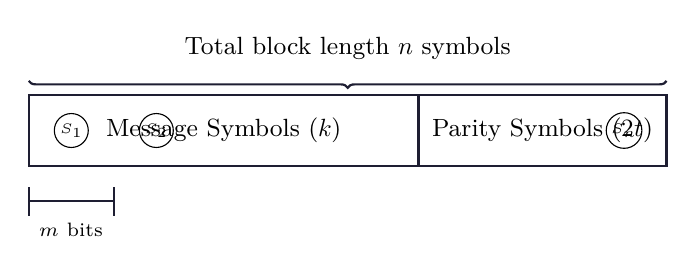
\begin{tikzpicture}[scale=0.9]
  \draw[line] (0,0) rectangle (9,1);
  \draw[line] (5.5,0) -- (5.5,1);
  
  \node at (2.75, 0.5) {\small Message Symbols ($k$)};
  \node at (7.25, 0.5) {\small Parity Symbols ($2t$)};
  
  \draw[line] (0, -0.3) -- (0, -0.7);
  \draw[line] (1.2, -0.3) -- (1.2, -0.7);
  \draw[line] (0, -0.5) -- (1.2, -0.5);
  \node at (0.6, -0.9) {\scriptsize $m$ bits};
  
  \node[draw, circle, inner sep=1pt] at (0.6, 0.5) {\tiny $S_1$};
  \node[draw, circle, inner sep=1pt] at (1.8, 0.5) {\tiny $S_2$};
  \node[draw, circle, inner sep=1pt] at (8.4, 0.5) {\tiny $S_n$};
  
  \draw[decoration={brace}, decorate, line, thick] (9, 1.2) -- (0, 1.2);
  \node[above=0.15cm] at (4.5, 1.2) {\small Total block length $n$ symbols};
\end{tikzpicture}
\end{tcolorbox}

\subsection{Error and Burst Correction Capability}
Since $d_{min} = n-k+1$, a Reed-Solomon code can correct up to $t$ symbol errors:
\[ t = \left\lfloor \frac{n-k}{2} \right\rfloor \]
RS codes are highly effective at correcting \textbf{burst errors} (consecutive bit errors). Since a symbol is treated as a single entity, if a burst of errors corrupts multiple bits within a single $m$-bit symbol, it counts as only \textbf{one symbol error}. A $t$-symbol correcting RS code can easily correct a continuous burst of errors up to $m(t-1) + 1$ bits.

% ===============================================================================
\section{MDS (Maximum Distance Separable) Codes}
% ===============================================================================

The Singleton bound states that for any linear block code with parameters $[n, k, d_{min}]$, the minimum distance is bounded by:
\[ d_{min} \le n - k + 1 \]

\begin{tcolorbox}[defbox, title={\textbf{MDS Code Definition}}]
A code is \textbf{Maximum Distance Separable (MDS)} if it meets the Singleton bound with strict equality:
\[ d_{min} = n - k + 1 \]
\end{tcolorbox}

\subsection{Properties of MDS Codes}
MDS codes are optimal because they achieve the maximum possible minimum distance for a given block length and code rate.
\begin{itemize}[leftmargin=*, itemsep=3pt]
  \item \textbf{Generator Matrix Independence:} A code is MDS if and only if \textbf{any $k$ columns} of its generator matrix $G$ are linearly independent.
  \item \textbf{Parity Matrix Independence:} A code is MDS if and only if \textbf{any $n-k$ columns} of its parity check matrix $H$ are linearly independent.
  \item \textbf{Dual Code:} The dual code of an MDS code is also an MDS code.
  \item \textbf{Examples:} Reed-Solomon codes are the most widely used class of MDS codes.
\end{itemize}

% ===============================================================================
\section{Justeen, Alterant and Goppa Codes}
% ===============================================================================

\subsection{Justeen Codes}
Justeen codes are a class of algebraic codes constructed by combining Reed-Solomon codes. They are designed to achieve good distance properties with simpler decoding algorithms.

\subsection{Alterant Codes}
Alterant codes are a generalization of BCH codes. They are defined by selecting roots from an extension field using a set of "locators" and "multipliers" that do not necessarily have the cyclic structure of standard BCH codes. This generalization allows for a wider choice of code lengths.

\subsection{Goppa Codes}
Goppa codes are an important class of non-cyclic algebraic codes defined by a \textbf{Goppa Polynomial} $g(z)$ over a finite field.
\begin{tcolorbox}[defbox, title={\textbf{Goppa Code Definition}}]
Let $L = \{\gamma_1, \gamma_2, \dots, \gamma_n\}$ be a set of distinct elements in $\text{GF}(2^m)$, and let $g(z)$ be a polynomial over $\text{GF}(2^m)$ such that $g(\gamma_i) \neq 0$ for all $i$. A Goppa code consists of all vectors $c = (c_1, \dots, c_n)$ that satisfy:
\[ \sum_{i=1}^n \frac{c_i}{z - \gamma_i} \equiv 0 \pmod{g(z)} \]
\end{tcolorbox}
Goppa codes are key to \textbf{code-based cryptography} (e.g., the McEliece cryptosystem) because their lack of cyclic structure makes them resistant to algebraic attacks while retaining strong error-correction capabilities.

\subsection{Generalized BCH Codes}
Generalized BCH codes extend standard BCH codes by relaxing the requirement that the roots be consecutive powers of a primitive element. By choosing an arbitrary set of roots, we can optimize the code for specific channels.

% ===============================================================================
\section{Code Classes Hierarchy}
% ===============================================================================

The relationship between the various algebraic code classes described can be represented as a hierarchical tree:

\begin{tcolorbox}[tikzbox, title={Algebraic Codes Hierarchy}]
\centering
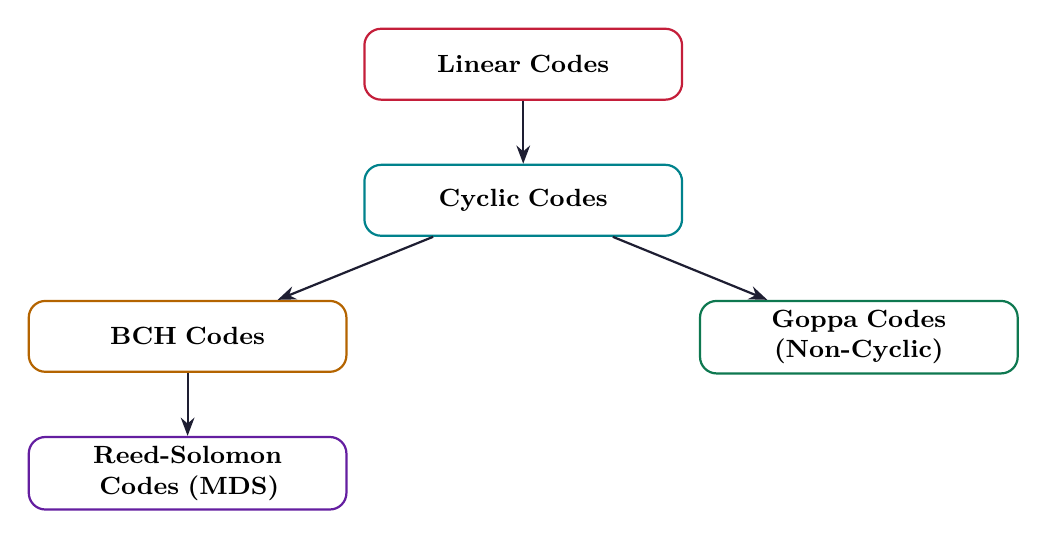
\begin{tikzpicture}[node distance=1.5cm and 0.5cm]
  \node[card, draw=myred] (lin) {Linear Codes};
  \node[card, draw=myteal, below=0.8cm of lin] (cyc) {Cyclic Codes};
  \node[card, draw=myamber, below left=0.8cm and 0.2cm of cyc] (bch) {BCH Codes};
  \node[card, draw=mygreen, below right=0.8cm and 0.2cm of cyc] (gop) {Goppa Codes (Non-Cyclic)};
  \node[card, draw=mypurple, below=0.8cm of bch] (rs) {Reed-Solomon Codes (MDS)};

  \draw[arrow] (lin) -- (cyc);
  \draw[arrow] (cyc) -- (bch);
  \draw[arrow] (cyc) -- (gop);
  \draw[arrow] (bch) -- (rs);
\end{tikzpicture}
\tcbset{after={\color{black}}}
\end{tcolorbox}

% ═══════════════════════════════════════════════════════════════════════════════
% QUICK REVISION PAGE
% ═══════════════════════════════════════════════════════════════════════════════
\newpage
\begin{center}
  {\large\bfseries\color{myred} Quick Revision --- Module 3}\\[3pt]
  {\small\color{mydark} BCH, RS and Special Codes $|$ PE-EC801C}
\end{center}
\noindent{\color{myred}\rule{\linewidth}{1.2pt}}
\vspace{4pt}

\begin{tcolorbox}[formulabox, title={\textbf{Key Formulas and Metrics at a Glance}}]
\renewcommand{\arraystretch}{1.35}
\begin{tabularx}{\linewidth}{B{5.0cm} X}
BCH roots criteria & $g(\alpha^i) = 0$ for $i = 1, 2, \dots, 2t$ \\[4pt]
BCH bound & $d_{min} \ge 2t + 1$ \\[4pt]
RS Block length (symbols) & $n = 2^m - 1$ \\[4pt]
RS Message length (symbols) & $k = n - 2t$ \\[4pt]
MDS Singleton equality & $d_{min} = n - k + 1$ \\[4pt]
RS Error correction capability & $t = \lfloor (n-k)/2 \rfloor$ symbol errors \\[4pt]
Idempotent condition & $e(x)^2 \equiv e(x) \pmod{X^n \oplus 1}$ \\[4pt]
Mattson-Solomon polynomial & $g_v(z) = \sum_{j=1}^n V_j z^{n-j}$ \\[4pt]
Goppa code congruence & $\sum_{i=1}^n \frac{c_i}{z - \gamma_i} \equiv 0 \pmod{g(z)}$
\end{tabularx}
\end{tcolorbox}

\vspace{6pt}

\begin{tcolorbox}[defbox, title={\textbf{One-Line Definitions}}]
\begin{itemize}[leftmargin=*, itemsep=3pt, topsep=0pt]
  \item \textbf{BCH Code:} A class of multiple-error-correcting cyclic codes defined by consecutive powers of $\alpha$ as roots.
  \item \textbf{Idempotent Polynomial:} A polynomial that is equal to its own square modulo $X^n \oplus 1$.
  \item \textbf{Reed-Solomon Code:} A non-binary subclass of BCH codes where symbols are from GF($2^m$).
  \item \textbf{Singleton Bound:} The upper limit on the minimum distance of a block code: $d_{min} \le n - k + 1$.
  \item \textbf{MDS Code:} A code that achieves the Singleton bound with equality.
  \item \textbf{Goppa Code:} A class of non-cyclic algebraic codes defined by a Goppa polynomial $g(z)$ over a finite field.
  \item \textbf{Burst Error:} A sequence of consecutive bit errors caused by channel disturbances.
  \item \textbf{Design Distance ($d_d$):} The lower bound on minimum distance ($2t+1$) used to construct a BCH code.
\end{itemize}
\end{tcolorbox}

\newpage

\begin{tcolorbox}[exambox, title={\textbf{Frequently Asked / Viva Questions}}]
\begin{enumerate}[topsep=0pt, label=\textbf{Q\arabic*.}, itemsep=5pt]
  \item \Q{How is a BCH generator polynomial constructed for a given error capability $t$?}
    We first identify the $2t$ consecutive roots: $\alpha^1, \dots, \alpha^{2t}$. Then, we find the minimal polynomials $m_i(x)$ for each of these roots. The generator polynomial is the least common multiple (LCM) of these minimal polynomials.
  \item \Q{Why are Reed-Solomon codes highly suited for burst error correction?}
    RS codes operate on $m$-bit symbols. An error burst of length $L$ bits can corrupt at most $\lceil L/m \rceil + 1$ symbols. Since correcting a symbol corrects all bit errors within it, RS codes handle localized burst corruptions very efficiently.
  \item \Q{What makes a code "Maximum Distance Separable" (MDS)?}
    A code is MDS if its minimum distance $d_{min}$ reaches the absolute theoretical maximum defined by the Singleton bound: $d_{min} = n - k + 1$. Reed-Solomon codes are the most famous example.
  \item \Q{Explain the role of the Goppa polynomial in cryptography.}
    Goppa codes are the foundation of McEliece cryptography. Because they lack cyclic structure, their generator matrices appear random to attackers, making it difficult to decode messages without the private Goppa polynomial.
  \item \Q{What is the difference between binary BCH codes and Reed-Solomon codes?}
    Binary BCH codes process individual bits, and their codewords consist of bits. RS codes are non-binary BCH codes where codewords consist of multi-bit symbols from GF($2^m$), offering better performance against symbol-level errors.
  \item \Q{What are idempotents and how do they relate to cyclic codes?}
    An idempotent is a polynomial satisfying $e(x)^2 \equiv e(x) \pmod{X^n \oplus 1}$. In cyclic codes, the generating idempotent serves as the identity element of the code and uniquely defines the ideal.
  \item \Q{Explain the Singleton bound and its implication.}
    The Singleton bound states $d_{min} \le n - k + 1$. It implies that the minimum distance cannot exceed the number of parity check bits plus one, representing the trade-off between redundancy and error capability.
  \item \Q{What are Justeen codes?}
    Justeen codes are algebraic codes built by combining Reed-Solomon codes, designed to achieve excellent distance properties with simpler, lower-complexity decoders.
  \item \Q{Define the Mattson-Solomon polynomial.}
    The Mattson-Solomon polynomial represents a vector as a polynomial $g_v(z) = \sum V_j z^{n-j}$ where $V_j$ are its finite field DFT coefficients, mapping time-domain data into the spectral domain.
  \item \Q{Is the actual minimum distance of a BCH code always equal to its design distance?}
    No. The BCH bound guarantees $d_{min} \ge 2t+1$. While the actual minimum distance is often equal to $2t+1$, it can sometimes be larger due to the properties of the minimal polynomials.
\end{enumerate}
\tcbset{after={\color{black}}}
\end{tcolorbox}

\vspace{6pt}

\begin{tcolorbox}[tikzbox, title={\textbf{Comparison of BCH and Reed-Solomon Codes}}]
\renewcommand{\arraystretch}{1.45}
\begin{tabularx}{\linewidth}{|B{3.2cm}|Y|Y|}
\hline
\textbf{Property} & \textbf{Binary BCH Codes} & \textbf{Reed-Solomon Codes} \\
\hline
Symbol Type & Binary bits ($0, 1$) & Non-binary symbols from $\text{GF}(2^m)$ \\
\hline
Block Length ($n$) & $2^m - 1$ bits & $2^m - 1$ symbols \\
\hline
Minimum Distance & $d_{min} \ge 2t + 1$ & $d_{min} = n - k + 1$ (MDS) \\
\hline
Error Target & Random single-bit errors & Burst errors and symbol-level corruptions \\
\hline
Complexity & Moderate & High (requires finite field arithmetic) \\
\hline
\end{tabularx}
\end{tcolorbox}

\end{document}
